上一節討論的是在同一臺機器上運行多個線程,而這些線程之間沒有任何交互。如果能以一種方式將程序所做的工作分割到多個線程之間,那麼無論如何都要這樣做。

線程之間通常需要交互,因為它們正在為一個共同的結果工作。這種交互是通過線程之間,通過共享資源(內存)進行通信的方式進行。我們現在必須理解這對性能的影響。

假設我們要計算多個值的和,有很多數字要累加,但最後只有一個結果,所以想要在幾個線程之間進行添加工作。因此線程在做加和時,結果值時必須進行交互。

\hspace*{\fill} \\ %插入空行
\noindent
\textbf{02\_sharing\_incr.C}
\begin{lstlisting}[style=styleCXX]
unsigned long x {0};
void BM_incr(benchmark::State& state) {
	for (auto _ : state) {
		benchmark::DoNotOptimize(++x);
	}
}
BENCHMARK(BM_incr)->Threads(2);
\end{lstlisting}

簡單起見,這裡將結果遞增1(整數相加的代價與值無關,並且不想對不同值的生成進行基準測試,而只想對加法進行基準測試)。由於基準函數由每個線程完成,因此在這個函數中聲明的任何變量都獨立存在於每個線程的堆棧上,這些變量不共享。為了得到兩個線程都參與的共同結果,變量必須在基準函數之外的文件範圍內聲明(這是個壞主意,但在微基準的非常有限的上下文中是必要和可接受的)。

當然,這個程序有一個比全局變量更大的問題:這是個錯誤的程序,其結果未定義。有兩個線程遞增相同的值,增加一個值需要3個步驟。程序從內存中讀取值,在寄存器中增加值,然後將新值寫回內存。兩個線程完全可以同時讀取相同的值(0),在每個處理器(1)上分別遞增,然後寫回。寫第二個線程的線程只是重寫第一個線程的結果,在兩次增量之後,結果是1,而不是2。這是因為兩個線程為了寫入同一內存位置而進行了競爭,這種競爭稱為\textbf{數據競爭}。

既然瞭解了為什麼這種無保護的併發訪問會出問題,那麼最好忘記它。相反,請遵循這個一般的規則:如果在沒有同步的情況下,讓多個線程訪問相同的內存位置,並且這些訪問中有一個是寫操作,結果是未定義的。這是非常重要的,沒有必要確切地指出必須做哪些操作序列會得到不正確的結果。事實上,在這種推理過程中什麼也得不到。當有兩個或更多的線程訪問同一個內存位置時,就會遇到數據競爭,除非能保證以下兩件事中的一件:要麼所有的訪問都只讀,要麼所有的訪問都使用了正確的內存同步(這一點我們還沒有了解到)。

計算求和的問題要求將結果寫入結果變量,所以訪問肯定不是隻讀的。內存訪問的同步通常由互斥鎖提供,每次訪問線程間共享的變量都必須由互斥鎖保護(當然,所有線程的互斥鎖必須相同)。

\hspace*{\fill} \\ %插入空行
\noindent
\textbf{03\_mutex\_incr.C}
\begin{lstlisting}[style=styleCXX]
unsigned long x {0};
std::mutex m;

{ // Concurrent access happens here
	std::lock_guard<std::mutex> guard(m);
	++x;
}
\end{lstlisting}

\texttt{lock\_guard}鎖在其構造函數中鎖定互斥鎖,並在析構函數解鎖。一次只有一個線程可以擁有鎖,這樣就可以對共享結果變量進行增加數值的操作。這時,其他線程被鎖阻塞,直到第一個線程釋放鎖後才能獲取鎖。注意,只要有一個線程在修改變量,所有的訪問(包括讀和寫)都必須阻塞。

鎖是確保多線程程序正確性的最簡單方法,但就性能而言,還挺難研究的。鎖的實現相當複雜,會經常涉及系統調用。我們將從一個同步選項開始,在這個特定的例子中,這個方式會更容易分析:原子變量。

C++提供了一個將變量聲明為原子變量的選項。這意味著對這個變量支持的所有操作都是不可中斷的原子事務。任何觀察這個變量的其他線程都將在原子操作前後看到它的狀態,但絕不會在操作的中間看到它的狀態。例如,C++中所有的整數原子變量都支持原子增量操作。如果線程正在執行這個操作,那麼在第一個操作完成之前,其他線程都不能訪問這個變量。這些操作需要一定的硬件支持,原子增量是一種特殊的硬件指令,它讀取舊的值,增加它的值,然後寫入新值,所有這些都作為一個單獨的硬件操作。

我們的示例中,只需要一個原子自增。必須強調的是,無論使用什麼同步機制,所有線程都必須使用相同的機制來併發訪問特定的內存位置。如果在一個線程上使用原子操作,只要所有線程都使用原子操作,就不存在數據競爭。如果另一個線程使用互斥鎖或非原子訪問,那保護不起作用,結果依舊是未定義的。

用C++的原子操作重寫基準測試:

\hspace*{\fill} \\ %插入空行
\noindent
\textbf{02\_sharing\_incr.C}
\begin{lstlisting}[style=styleCXX]
std::atomic<unsigned long> x(0);
void BM_shared(benchmark::State& state) {
	for (auto _ : state) {
		benchmark::DoNotOptimize(++x);
	}
}
\end{lstlisting}

程序現在是正確的,這裡沒有數據競爭。這並不一定準確,因為單個自增是在一個非常短的時間間隔內進行的,這裡應該手動展開循環或使用宏,並在每次循環迭代中進行多次遞增(已經在上一章中做了這一點,所以可以在那裡看到這樣的宏)。若線程之間沒有交互,兩個線程計算總和的時間將是一個線程計算總和的一半:

%\hspace*{\fill} \\ %插入空行
\begin{center}
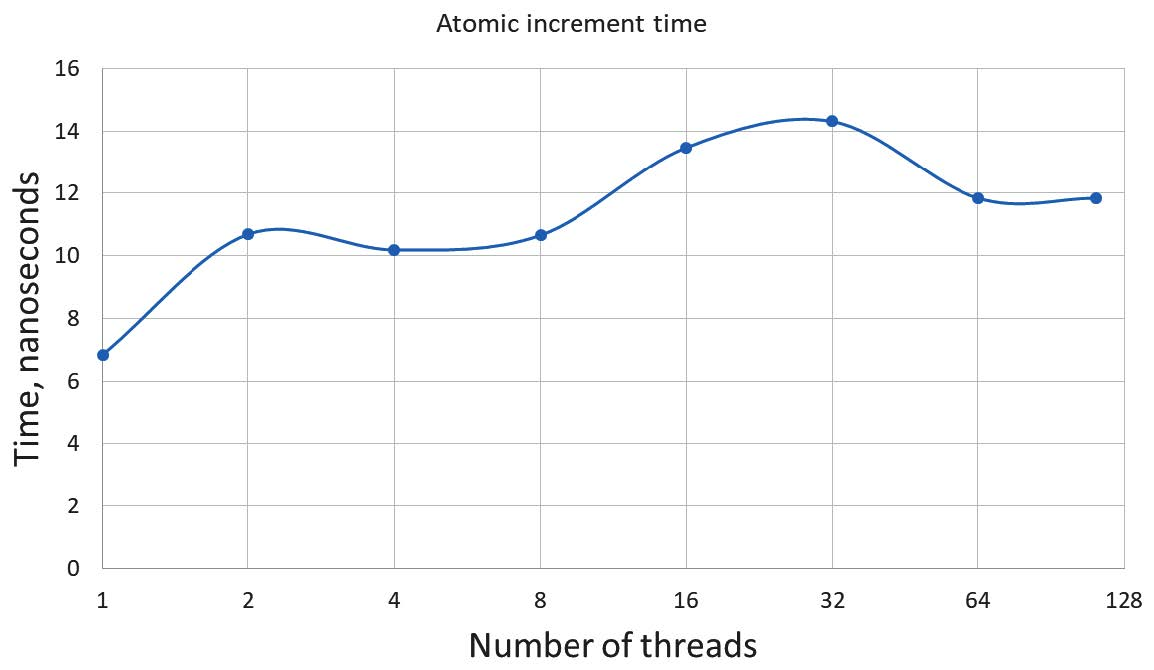
\includegraphics[width=0.9\textwidth]{content/1/chapter5/images/4.jpg}\\
圖5.4 - 多線程程序中原子自增的時間
\end{center}

對結果進行了標準化,以顯示單個增量的平均時間,即計算和除以相加總數的時間。這個程序的性能非常令人失望,不僅沒有任何改進,在兩個線程上計算總和要比在一個線程上花費更長的時間。

如果使用互斥鎖,結果會更糟:

%\hspace*{\fill} \\ %插入空行
\begin{center}
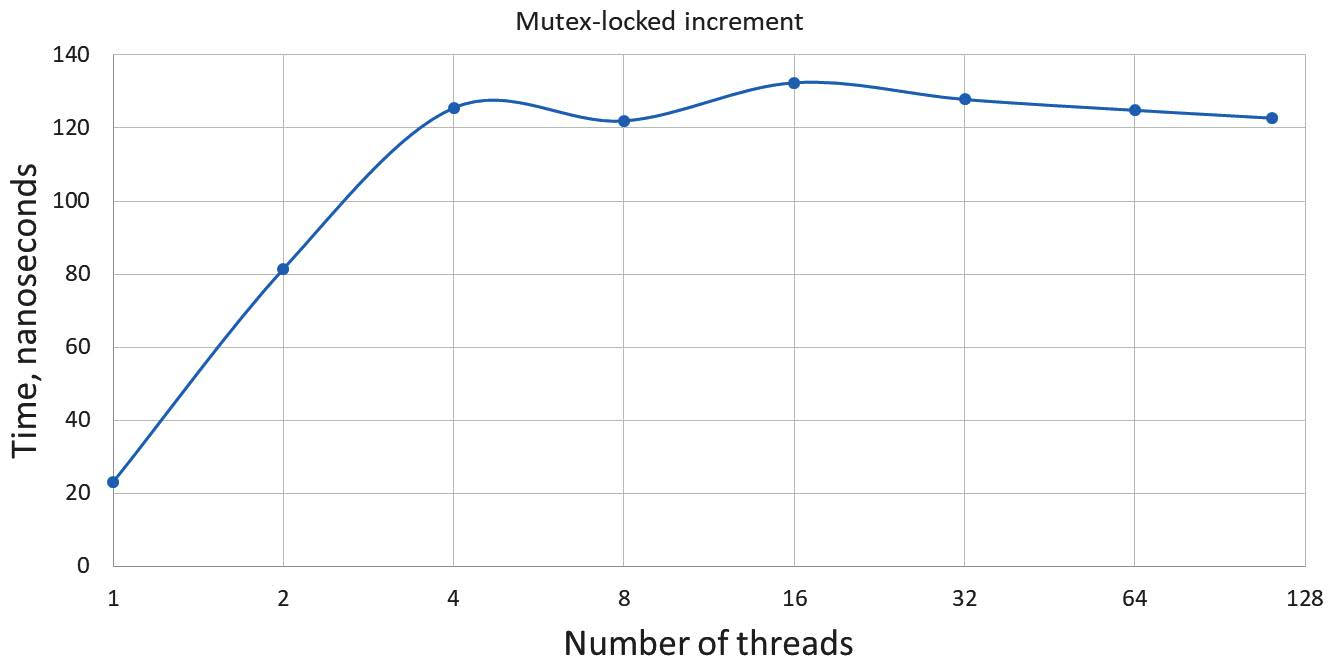
\includegraphics[width=0.9\textwidth]{content/1/chapter5/images/5.jpg}\\
圖5.5 - 多線程程序中使用互斥量會增加耗時
\end{center}

首先,鎖定互斥鎖是一個相當耗時的操作,即使在一個線程上。互斥鎖需要23納秒,而原子變量需要7納秒。隨著線程數量的增加,性能會下降得更快。

可以從這些測試中瞭解到很多。程序中訪問共享數據的部分永遠不會擴展,訪問共享數據的最佳性能是單線程性能。當有兩個或更多的線程同時訪問相同的數據,性能只會變得更糟。當然,如果兩個線程在不同的時間訪問相同的數據,它們不會交互,因此兩次都獲得了單線程性能。多線程的性能優勢來自於線程獨立計算,而不需要同步。這樣的計算可以在不共享的數據上進行(無論如何,若希望程序結果正確),但是為什麼對共享數據的併發訪問有如此大的開銷呢?下一節中,我們將瞭解其中原因,也將瞭解如何解析測試結果。








